We hereby present a first proof-of-concept for a CarPal application
implementing the concepts exposed above.  The software is still at an
initial development but it has already been proven to be working in
posting new routes and querying them across multiple networks.  A
basic user interface is proposed showing a first attempt to integrate
a mapping service (namely, Google Maps \cite{googlemaps:website}) in
the application, to render the user experience more pleasant and
efficient.
 
%
\subsection{Building the scenario}
%
Let's see a practical example to better explain the logic behind the
application.  As a real world scenario for our proof-of-concept we
chose the area area of Sophia Antipolis in the department of
Provence-Alpes-Cote d'Azur, France. The area (Figure \ref{tab:journey}
left) constitutes an ideal study case, being a technological pole with
a high concentration of IT industries and research centers, thus
providing several potential communities of people working in the same
area and living in nearby towns (Antibes, Nice, Cagnes sur Mer to name
some).
 

An engineer working in the area and willing to do some car pooling in
order to reduce his daily transfer costs can publish his usual route
to the CarPal overlay specific to his company. We assume the network
has been already put in place spontaneously by him or some colleague
of his.  He can then use the CarPal application to publish his route
with an intermediate checkpoint (as shown in Figure
\ref{fig:publish1}).
%
\begin{figure}
  \begin{center}
    \begin{tabular}{c@{\hspace{2mm}}c}
      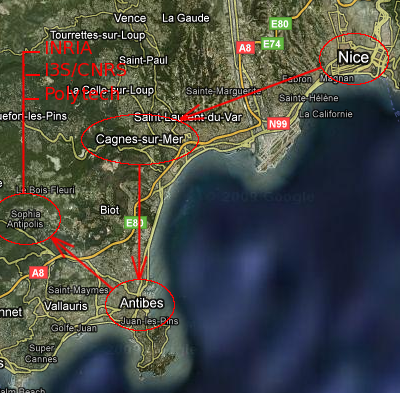
\includegraphics[scale=0.38]{fig/screenshot/geolock2}
      &
      \begin{tabular}[b]{l}
        \begin{tabular}{|l|l|} \hline 
          Trip date & 15/01/2010 \\ \hline 
          Departure & Nice \\ \hline 
          Departure Time & 8.00 \\ \hline
          Checkpoint & Cagnes sur Mer \\ \hline 
          Checkpoint Time & 8.30 \\ \hline
          Arrival & Sophia Antipolis \\ \hline 
          Arrival Time & 9.00 \\ \hline
          Seats available & 4 \\ \hline 
          Contact & jsmith@email.com \\ \hline
        \end{tabular}
        \\\\
        \begin{tabular}[b]{|l|l|} \hline 
          Nice-Sophia & 8.00-9.00 \\ \hline
          Nice-Cagnes sur Mer & 8.00-8.30 \\ \hline
          Cagnes sur Mer-Sophia & 8.30-9.00 \\ \hline
        \end{tabular}
      \end{tabular}
    \end{tabular}
  \end{center}
  \caption{The ``Geo'' set-up and the journey data (right) and sliced / diced segments (bottom right)}
  \label{tab:journey}
\end{figure}
%
\begin{figure}[!t]
\begin{center}
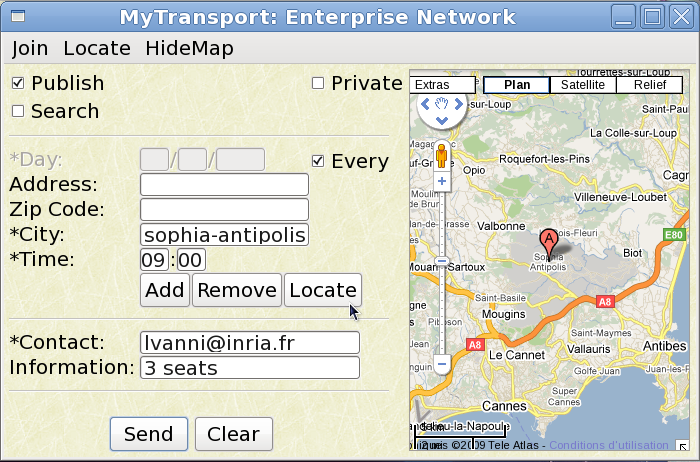
\includegraphics[scale=0.4]{fig/screenshot/enterprisePub}
\end{center}
\caption{CarPal application publishing a new trip}
\label{fig:publish1}
\end{figure}
%
As previously described, there is a checkpoint where our user
is willing to stop and pick up some passengers.

\subsection{Slice and Dice and encoding in the DHT}
%
Starting from the above data all the possible combinations are
generated leading to the segments shown in Figure \ref{tab:journey}
(right). Only the differences are reported, each of those segments
share the same date, available seats and contact information.  The 3
segments are then stored in the DHT by updating the appropriate keys
or adding new ones, as shown in Table \ref{tab:keys}.  Time and dates
are converted to appropriate strings while geographical positions are
identified by a placeholder (\ie\ \key{NICE}, \key{SOPH}...)
representing a record accessible in the DHT or the central tracker.
%
\begin{table}
  \begin{center}
    \key{\small{
        \begin{tabular}{|c|l|l|c|}
          \hline
          \bf{Criteria} & \multirow{2}{*}{\bf{Operation}} & \multirow{2}{*}{\bf {Key}} & \multirow{2}{*}{\bf {Value}} \\ 
          \bf{(see Table \ref{t:DHTvalues})} & & & \\ \hline
          1 & PUT & TR 123 & $\clubsuit$ \\ \hline
          1 & PUT & TR 124 & $\spadesuit$ \\ \hline
          1 & PUT & TR 125 & $\blacksquare$ \\ \hline
          2 & APPEND & T 20100115 NICE 0800 SOPH 0900 & 123 \\ \hline
          2 & APPEND & T 20100115 NICE 0800 CAGN 0830 & 124 \\ \hline
          2 & APPEND & T 20100115 CAGN 0830 SOPH 0900 & 125 \\ \hline
          3 & APPEND & DA 20100115 NICE SOPH & 123 \\ \hline
          3 & APPEND & DA 20100115 NICE CAGN & 124 \\ \hline
          3 & APPEND & DA 20100115 CAGN SOPH & 125 \\ \hline
          4 & APPEND & D 20100115 NICE & 123 \\ \hline
          4 & APPEND & D 20100115 NICE & 124 \\ \hline
          4 & APPEND & D 20100115 CAGN & 125 \\ \hline
          5 & APPEND & A 20100115 SOPH & 123 \\ \hline
          5 & APPEND & A 20100115 CAGN & 124 \\ \hline
          5 & APPEND & A 20100115 SOPH & 125 \\ \hline
          6 & APPEND & U jsmith@email.com & [123,124,125] \\ \hline
        \end{tabular}
      }}
  \end{center}
  
where $\clubsuit$ = [20100115, NICE, 0800, SOPH,0900, 3, jsmith@email.com, public=true] \\
where $\spadesuit$ = [20100115, NICE, 0800, CAGN,0830,3, jsmith@email.com, public=true] \\
where $\blacksquare$ = [20100115, CAGN, 0830, SOPH, 0900, 3, jsmith@email.com, public=true] \\
\caption{DHT operations}
  \label{tab:keys}
\end{table}

A PUT operation represents the insertion of a new key not yet existing
whereas the APPEND operation assumes that the key might be already in
the DHT, in which case the value is simply updated by adding the new
entry to the list.
After the insertion the trip is published and available to be
searched. From Figure \ref{fig:publish1} we can see that it's possible
to set as an option that the trip will stay private.  In that case,
the segments will be discoverable only by peers members of the same
network.

\subsection{Searching for a trip}
%
Trip searching happens in a similar way as the trip submission. As we
can see in Figure \ref{fig:searchAggregate} (left) the user can
specify an itinerary, a specific time and even some intermediate
segments to find all the possible combinations. Depending on the
search criteria specified, the application will perform a query for
either a key made of Time of Departure and Time of Arrival, for a more
exact match, a key with only Departure and Arrival to browse through
the day's trips or a key with only Departure or Arrival point for a
broader search.  Thanks to the Slice and Dice operation it is possible
to aggregate segments coming from different users as Figure
\ref{fig:searchAggregate} (right) shows.

\begin{figure}[!t]
\begin{center}
\mbox{\rew{10}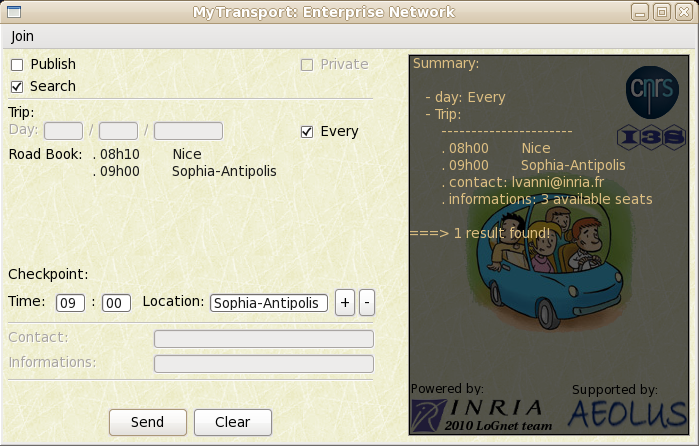
\includegraphics[scale=0.3]{fig/screenshot/NiceSophiaSub}
~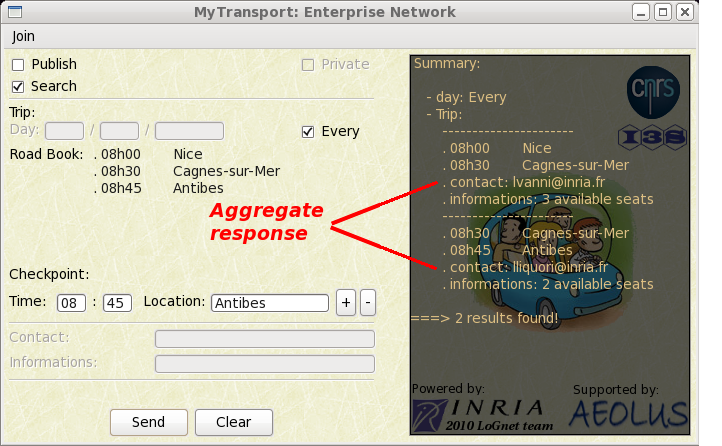
\includegraphics[scale=0.3]{fig/screenshot/NiceCagnesAntibesSub}}
\end{center}
\caption{Simple search \vs\ aggregate results}
\label{fig:searchAggregate}
\end{figure}

This way the driver has more possibilities to find guests in his
car. Despite that there can still be some places available for his
daily route. To optimize even further he might share his information
with, for example, students of nearby universities with their own
carpool network (that has the same functions and technology).

By marking his published itinerary as public, a member of the
Enterprise Network allow the students to get matching results via a
synapse (Figure \ref{fig:searchForeign}), \ie\ somebody registered to
both networks (Figure \ref{fig:studententerprise}).  This allows the
system to increase the chances of finding an appropriate match while
maintaining good locality properties.

\begin{figure}[!t]
\begin{center}
\mbox{\rew{15}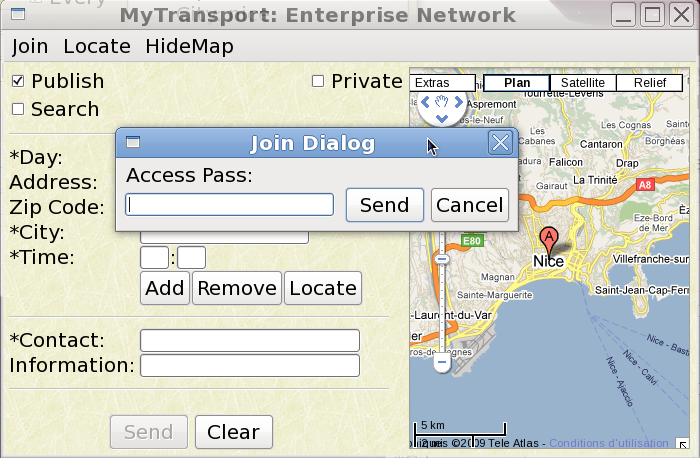
\includegraphics[scale=0.3]{fig/screenshot/EnterpriseJoinStudent}~
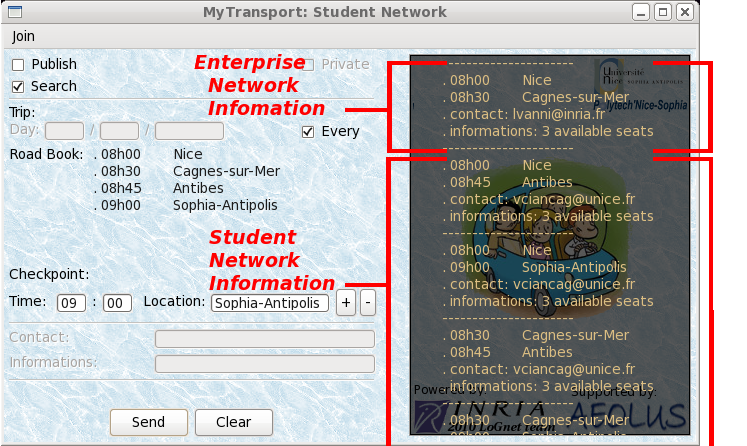
\includegraphics[scale=0.31]{fig/screenshot/NiceCagnesAntibesSophiaSub_StudentNetwork}}
\end{center}
\caption{Synapse creation (left). CarPal Students accessing result from Enterprise Network (Right)}
\label{fig:searchForeign}
\end{figure}

 
\begin{figure}[!t]
\begin{center}

\includegraphics[scale=0.3]{fig/screenshot/Student-Enterprise}
\\[-10mm]

\includegraphics[scale=0.3]{fig/screenshot/Synapse-Network}
\end{center}
\caption{Students, Enterprise and Synapsed Overlay Networks}
\label{fig:studententerprise}
\end{figure}

 
